\documentclass[12pt]{article}

% This is documentation for the `edmaths` LaTeX package, maintained by
% Josh Fogg for the University of Edinburgh. This file closely builds on
% that provided Alan Munn for the MSU Thesis Class, `msu-thesis`. The
% original documentation is licensed under LaTeX Project Public License
% (LPPL) version 1.3 or later, and this documentation is licensed under
% the LLP version 1.3c. For more information, see the GitHub repository:
% https://github.com/Foggalong/edinburgh-math-latex

\def\msuversion{0.99}
\def\msudate{2024-08-30}
\title{\textbf{Using the \pkg{beamertheme-edmaths} Beamer Theme}}
\author{\textbf{Josh Fogg}\\School of Mathematics\\The University of Edinburgh\\\texttt{\href{mailto:j.fogg@ed.ac.uk}{j.fogg@ed.ac.uk}}}
\date{Version \msuversion\\\msudate}

% basic formatting tweaks
\usepackage[lmargin=2cm,rmargin=2cm,tmargin=3cm,bmargin=2cm]{geometry}
\usepackage[colorlinks=true]{hyperref}
\usepackage{enumitem}
\usepackage{graphicx}

% use same fourier font available through edmaths
\usepackage{cmap}
\usepackage{fourier}
\usepackage[T1]{fontenc}
\usepackage{microtype}

% setup syntax highlighting
\usepackage{highlightlatex}
\definecolor{whiteF0}{HTML}{F0F0F0}
\lstset{
    % external padding
    aboveskip=.4em,
    belowskip=-.2em,
    xleftmargin=.03\textwidth,
    xrightmargin=.03\textwidth,
    % basic formatting
    backgroundcolor=\color{whiteF0},
    showstringspaces=false,
    columns=fixed,
    basewidth=.5em,
    basicstyle={\fontfamily{zlmtt}\selectfont},
    breaklines=true
}


% change new paragraph behaviour to no-indent and a linebreak
\usepackage[parfill]{parskip}


\newcommand\pkg[1]{\href{https://www.ctan.org/pkg/#1}{\color{teal}\lstinline{#1}}}
\newcommand\key[1]{{\color{orange}\lstinline|#1|}}


\begin{document}
\maketitle
\thispagestyle{empty}

\section{Introduction}

This is theme for \pkg{beamer}, used to creating presentations for the \href{https://www.maths.ed.ac.uk/}{School of Mathematics} at the \href{https://www.ed.ac.uk/}{University of Edinburgh}. It's designed as an accompaniment to \pkg{edmaths} and provides an easy way to generate a presentation in \LaTeX{} which aligns the university brand guidelines. This means you can focus on your actual writing, rather than worrying about font spacing, margins sizes, {\it etc}.

\section{Initial Setup}

This theme is designed to work with \pkg{beamer}, which should be available with any \TeX{} distribution. It can be used with any \LaTeX{} engine, including pdfLaTeX, XeLaTeX, or LuaLaTeX. While it should work with any reasonably up-to-date \TeX{} distribution, it is tested with 2020 and later.

The essential steps to setup are then:
\begin{enumerate}
    \item Choose a document class using \lstinline|\documentclass[<options>]{beamer}|, with \key{<options>} being defined in the full \pkg{beamer} documentation.
    \item Apply the theme using \lstinline|\usetheme{edmaths}|.
    \item Use \lstinline|\title[Short Title]{Full Title}|| to define the title (the \key{Short Title} is optional).
    \item Set the optional \lstinline|\subtitle{...}| if desired.
    \item Set the \lstinline|\author{...}| and \lstinline|\date{...}|.
\end{enumerate}
These steps {\bf must} be done in exactly this order or the compiler will throw errors.

Unlike \pkg{edmaths}, this theme does not automatically load the standard suite of \LaTeX{} math packages ({\it e.g.\/} \pkg{amsmath}) so you may wish to load those. Instead it loads \pkg{amsfonts}, \pkg{graphicx}, \pkg{lmodern}, and \pkg{mathptmx} which are necessary for the theme.

The basic package has no other special requirements, but if you have certain additional packages installed then you can use some fancifying options (see below).

\section{Package Options}

When loading \pkg{beamertheme-edmaths} with
\begin{lstlisting}
\usetheme[<options>]{edmaths}
\end{lstlisting}
we can supply additional \key{<options>} as a comma-separated list of the following keywords.

\subsection{Colour}

The default theme is styled around University of Edinburgh {\bf\color[HTML]{00325F} blue (\lstinline|#00325F|)}. It's also available in three other official brand colour-scheme variations by specifying at most one of:
\begin{itemize}
    \item \key{colour=UoEorange} for {\bf\color[HTML]{CC5911} orange (\lstinline|#CC5911|)},
    \item \key{colour=UoEgreen} for {\bf\color[HTML]{9C9A00} green (\lstinline|#9C9A00|)},
    \item \key{colour=UoEcyan} for {\bf\color[HTML]{457E81} cyan (\lstinline|#457E81|)}.
\end{itemize}
In theory other off-brand colours could be applied using \pkg{xcolor} and the same syntax, but this isn't officially supported so results may vary.

\subsection{Title Height}

By default the title height is \key{10ex}. This can be modified by specifying \key{theight=<x>}, where \key{<x>} is the desired height in a \LaTeX{} compatible unit.

\section{Usage}

Once \pkg{beamertheme-edmaths} is set up, a simple example of how it might be put together in \pkg{beamer} is in the listing below. A more complicated example is packaged with \pkg{beamertheme-edmaths} and \href{https://github.com/Foggalong/edinburgh-math-latex/blob/main/example-presentation.tex}{available here}. What this looks like compiled can be \href{https://foggalong.github.io/edinburgh-math-latex/example-presentation.pdf}{viewed here}.

\subsection{Overleaf}

As a student or staff member at the University of Edinburgh you have access to \href{https://www.ed.ac.uk/information-services/computing/desktop-personal/software/main-software-deals/other-software/overleaf}{Overleaf Professional}! Do make use of this, it alleviates many of the headaches which come with using \LaTeX{} across multiple computers, which you surely will..

\subsection{Archiving your presentation for the future}

The current version of \pkg{beamertheme-edmaths} satisfies the brand guidelines at any one time. Given these change, you may find that if you need to recompile your presentation later that the formatting changes. To avoid this, save an archived version of the \href{https://github.com/Foggalong/edinburgh-math-latex/blob/main/beamerthemeedmaths.sty}{\lstinline|beamerthemeedmaths.sty|} file in the same folder as your slides. You only need to do this once you have completely finished your presentation however; there's no need to do it during the writing process.

\begin{lstlisting}[caption={Example usage of \pkg{beamertheme-edmaths}.}]
\documentclass{beamer}
\usetheme{edmaths}

\title[Short Title]{A Long and verbose title}
\subtitle{and a sub-title}  % optional
\author{Dr Benway}
\institute{The Mental Institute}  % optional
\date{Feb 1935}

\begin{document}

\maketitle

\begin{frame}{Words of Advice for Young People}\label{sec:Advice}
    People often ask me if I have any words of \alert{advice} for
    young people\ldots \\[2ex] \pause
    \begin{itemize}
        \item<1-> \alert{Never} interfere in a \alert{boy-and-girl}
                  fight
        \item<2-> Any \alert{old soul} is worth saving \\
                  \uncover<3->{at \alert{least to} a priest},
            \begin{itemize}
                \item<4-> But \alert{not} every soul is \alert{worth
                          buying}.
            \end{itemize}
        \item<5-> \ldots
    \end{itemize}
\end{frame}

\begin{frame}{Conclusions}\label{sec:what?}
    \begin{itemize}
        \item<2-> What \alert{are} we doing here?
        \item<4-> What?
        \item<2-> Answers:
            \begin{itemize}
                \item<3-> We are here \alert{to go}.
            \end{itemize}
    \end{itemize}
\end{frame}

\end{document}
\end{lstlisting}

\section{Speaker Notes}

There are various solutions for writing notes to accompany LaTeX presentations made with \pkg{beamer}. In each of these use the relevant command {\it after} the slide you wish to annotate.

\subsection{Beamer's \texttt{note}}

Core \pkg{beamer} itself actually comes with a command, \lstinline|\note|, which can be used for writing notes that are then included as separate `notes' pages in the complied PDF. Exactly how these are handled is controlled through the document class arguments

\begin{lstlisting}
\documentclass[notes]{beamer}       % print frame + notes
\documentclass[notes=only]{beamer}  % only notes
\documentclass{beamer}              % only frames    
\end{lstlisting}

and then notes are added with

\begin{lstlisting}
\begin{frame}
    ...
\end{frame}
\note{Some wonderful note.}
\end{lstlisting}

These have the upside that you have full access to \LaTeX{} formatting when writing your speaker notes, but the downside that they can be cumbersome to work with when presenting. Multiple complications are needed to get notes and presentations in separate PDF files.

\subsection{PDFPC's \texttt{note}}

\href{https://pdfpc.github.io/}{PDFPC} is a presenter console with multi-monitor support for PDF files. There's an official package, \pkg{pdfpc}, for adding meta-data to presentation files which are compatible with their presenter console. The screenshot in Figure~\ref{fig:pdfpc} shows how the console looks when viewing the example presentation.

\begin{figure}
    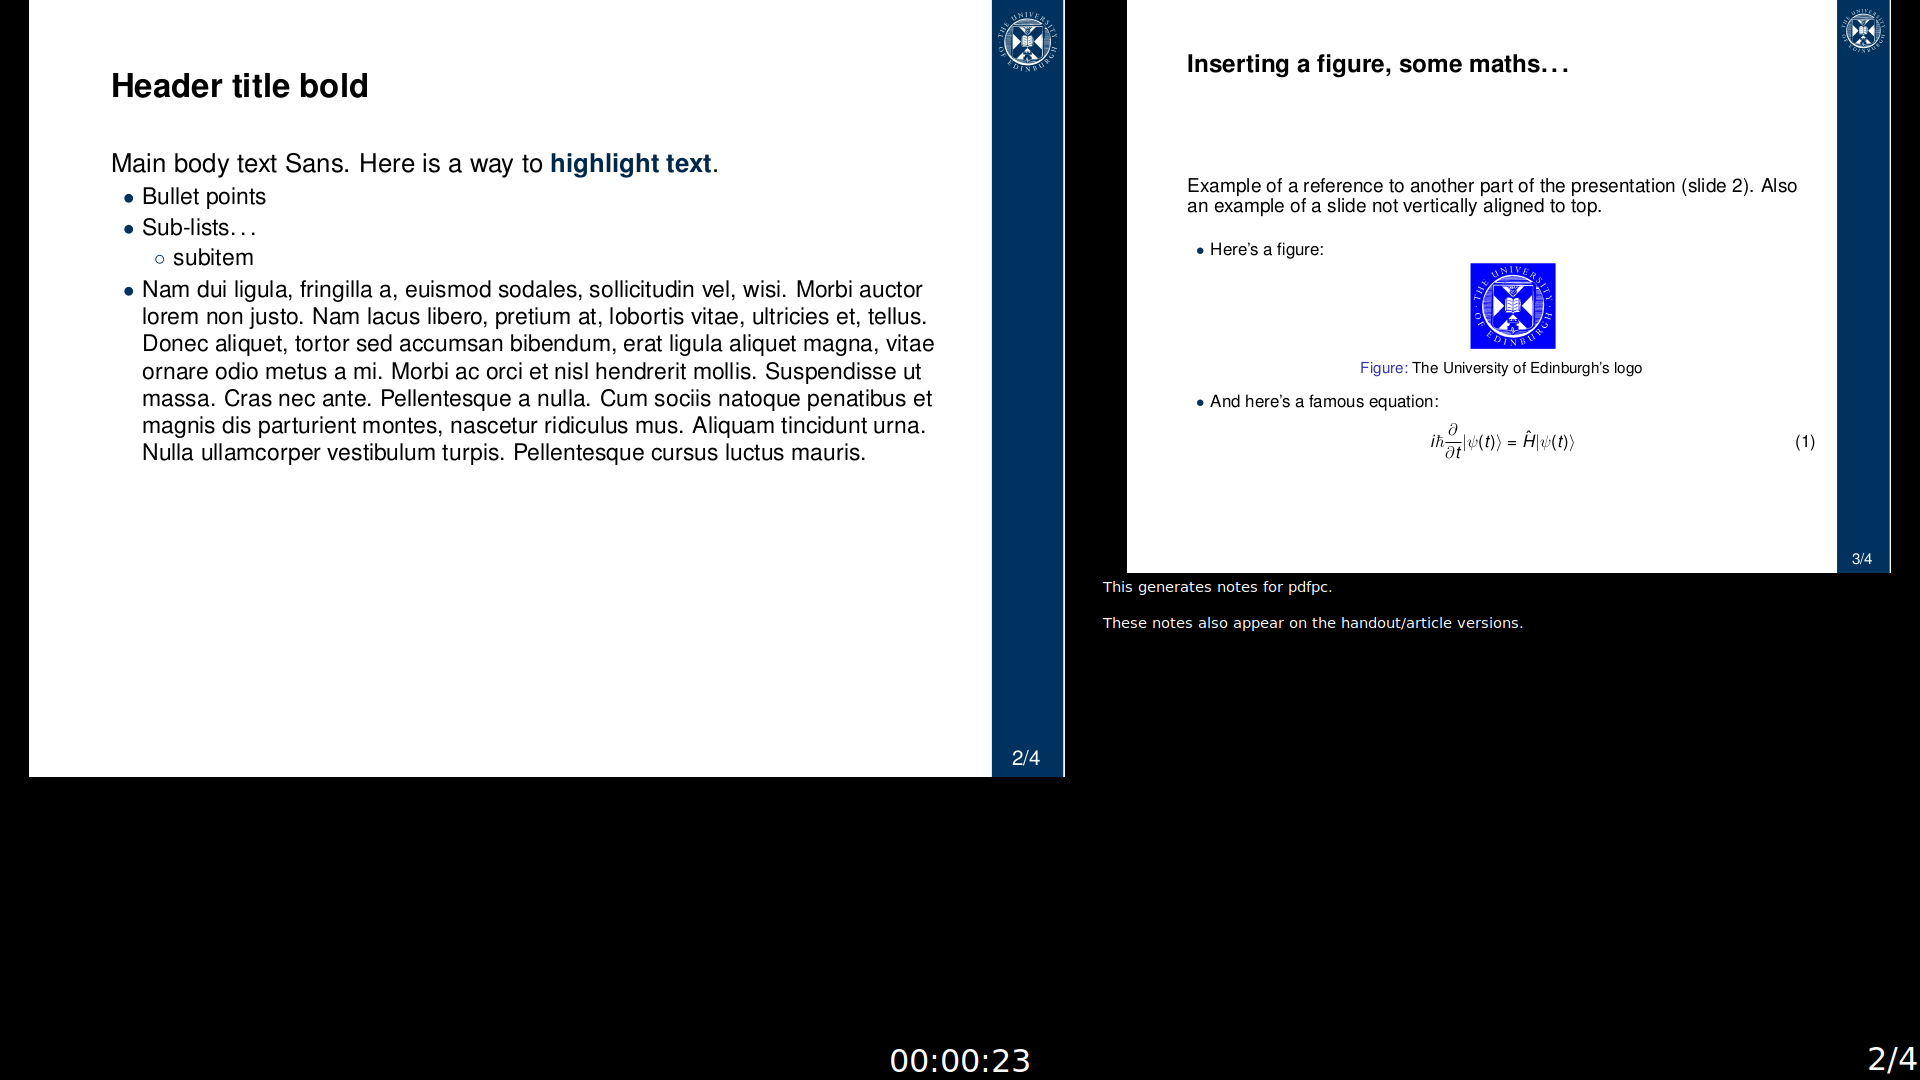
\includegraphics[width=\textwidth]{pdfpc-screenshot.png}
    \caption{Speaker notes in PDFPC.}\label{fig:pdfpc}
\end{figure}

To use this add

\begin{lstlisting}
\usepackage[overridenote=true]{pdfpc}  
\end{lstlisting}
and then it's just \lstinline|\note{Some wonderful note.}| as before.

These will then be included as ``comments'' within the complied PDF which PDFPC displays as notes in the presenter console. These have the upside that they're smoother to work with when presenting, but the downside that the only formatting supported is \lstinline|\\| for newlines.

\subsection{Brandt's \texttt{pnote}}

There are two packages called \pkg{pdfpc-latex-notes}, one by \href{https://github.com/cebe/pdfpc-latex-notes}{Carsten Brandt} and a fork by \href{https://github.com/p4pyru5/pdfpc-latex-notes}{p4pyru5}. These both generate PDFPC compatible notes using \lstinline|\pnote{Some wonderful note.}|. They served as the inspiration for PDFPC's official solution, but each come with their own (varying support for formatting, wider integration, {\it etc\/}).

\subsection{Usher's \texttt{bnote}}

The original version of the University of Edinburgh \pkg{beamer} template by \href{https://www.ed.ac.uk/profile/saturnino-luz}{Saturnino Luz} at the \href{https://www.ed.ac.uk/usher}{Usher Institute} included its own package, \pkg{beamernotes}, for generating a PDFPC compatible notes file.

To use it save \href{https://github.com/Foggalong/edinburgh-math-latex/blob/4ac2ffb765a7d9dc420396dd10bdafcc0c561398/beamernotes.sty}{\texttt{beamernotes.sty}} either to your \LaTeX{} path or local to your project. Then add

\begin{lstlisting}
\usepackage{beamernotes}  
\end{lstlisting}

to your document header and use

\begin{lstlisting}
\bnote{Some wonderful note.}  
\end{lstlisting}

to write your notes. This solution had the upside that your notes were included in a separate file still automatically read by PDFPC, but the downside that all formatting was lost {\it including} the ability to write newlines.

\section{Acknowledgements}

The original \pkg{beamertheme-edmaths} was written by \href{https://www.ed.ac.uk/profile/saturnino-luz}{Saturnino Luz} for \href{https://www.ed.ac.uk/usher}{Usher}, then modified by \href{https://github.com/bencwbrown}{Ben Brown} with general university branding. Both are freely provided under the terms of the \href{https://choosealicense.com/licenses/lppl-1.3c/}{\LaTeX{} Project Public License v1.3c} and from 2020 onwards have been maintained by \href{https://www.maths.ed.ac.uk/~jfogg/}{Josh Fogg} (me).

If you have any issues using \pkg{beamertheme-edmaths} don't hesitate to get in touch either by \href{mailto:j.fogg@ed.ac.uk}{email} or on \href{https://github.com/Foggalong/edinburgh-math-latex/issues/new?assignees=&labels=pres&projects=&template=beamer-issue.md&title=}{GitHub}. Feel free pop me a message just to say hi too, it always makes my day!

\end{document}